\documentclass[conference]{IEEEtran}
\IEEEoverridecommandlockouts

\usepackage{graphicx}
\usepackage{booktabs}
\usepackage{url}
\usepackage{amsmath}
\usepackage{array}
\usepackage{fancyhdr}

\pagestyle{fancy}
\fancyhf{}
\cfoot{\thepage}
\renewcommand{\headrulewidth}{0pt}

\newcommand{\figplaceholder}[1]{\fbox{\parbox[c][#1][c]{0.92\columnwidth}{\centering figure placeholder}}}
\newcommand{\figplaceholderwide}[1]{\fbox{\parbox[c][#1][c]{0.95\textwidth}{\centering figure placeholder}}}

\begin{document}

\title{A Comparison of $k$-Nearest Neighbours and Classification Trees for
Multi-Class Network Intrusion Detection}

\author{\IEEEauthorblockN{G. Scott}
\IEEEauthorblockA{Student number: 25935453\\
Email: 25935453@sun.ac.za}}

\maketitle

% ============================================================
\begin{abstract}
Network intrusion detection is posed here as a multi-class classification
problem, where each instance describes a single network connection labelled
as normal traffic or as one of nine attack categories. The class distribution
is heavily skew, and the rare attack categories are the ones an intrusion
detector most needs to find. This report builds, tunes and compares a
$k$-nearest neighbours classifier and a classification tree on such a
dataset. Pre-processing was decided separately for each model, because a
distance-based learner and a classification tree are not affected equally by
the same data quality issue. Control parameters were tuned by grid search on
a pool of instances held disjoint from the evaluation data, and both models
were then evaluated by ten-fold stratified cross-validation on the remaining
instances over identical folds. The classification tree recorded the higher
macro-averaged F1, won every fold, and the difference survived a corrected
resampled $t$-test. The ordering reversed on plain accuracy, so the better
model depends on the value placed on the rare categories. Conflicting target
levels on identical feature vectors also place a ceiling on macro-averaged
F1. Neither model came close to that ceiling, so the gap between the two
models is smaller than the gap between either model and the limit of the
data.
\end{abstract}

% ============================================================
\section{Introduction}

Network intrusion detection separates normal network traffic from attack
traffic, and the task suits supervised classification. Labelled historical
traffic is available for training, and new connections arrive continuously for
classification. The dataset holds 257\,673 instances, each describing a single
network connection through 43 descriptive features. The target feature records
normal traffic or one of nine attack categories, and the class distribution is
heavily skew, with the largest level holding 534.5 times as many instances as
the smallest. Several data quality issues also remain, including missing
values, strong correlations, large positive outliers, numeric ranges spanning
several orders of magnitude, a unique identifier and three nominal features.

The goal of this assignment is to build, tune and compare two classification
models on the dataset. The first model is $k$-nearest neighbours (kNN), and the
second is a classification tree. The two algorithms rest on different
assumptions, so the same data quality issue does not affect them equally, and
pre-processing was therefore decided separately for each model.

For both models the control parameters were tuned by grid search on a pool of
30\,000 instances, held disjoint from the data used for evaluation. The models
were then evaluated by ten-fold stratified cross-validation on the remaining
227\,673 instances. Performance was measured primarily by macro-averaged F1,
which gives every target level equal weight. The tree reached 0.5749 against
0.4975 for kNN and won on every fold. The ordering reverses on plain accuracy,
so the better model depends on the value placed on the rare attack categories.
A third figure frames both scores: 15.7\% of instances share a feature vector
with an instance carrying a different label, so a macro-averaged F1 above
0.7759 is unreachable.

The remainder of the report is organised as follows: Section~\ref{sec:background}
describes the two classification algorithms and states the expectations regarding
the remaining data quality issues. Section~\ref{sec:method} describes the
implementation and the pre-processing applied to each model.
Section~\ref{sec:empirical} describes the empirical procedure.
Section~\ref{sec:results} reports and discusses the results, and
Section~\ref{sec:conclusion} concludes the report.

% ============================================================
\section{Background}
\label{sec:background}

This section provides the background required for the remainder of the report.
Section~\ref{sec:algorithms} describes the two classification algorithms at a
high level. Section~\ref{sec:expectations} states the expected impact of each
remaining data quality issue on each of the two algorithms.

\subsection{Similarity-Based and Information-Based Classification}
\label{sec:algorithms}

Similarity-based learning predicts the target level of a query instance by
finding the most similar instances in a labelled dataset \cite{topic3}. The kNN
algorithm is the standard example. Training consists only of storing the
dataset, so kNN is a lazy learner \cite{kelleher2015}. A prediction is made by
measuring the distance from the query to every stored instance, selecting the
$k$ closest, and returning the majority target level among them
\cite{topic3,kelleher2015}.

Distance is measured using a metric from the Minkowski family, where a
parameter value of one gives the Manhattan distance and a value of two gives
the Euclidean distance \cite{topic3,kelleher2015}. Euclidean distance squares
each per-feature difference, so one large difference has a strong effect on the
result. Manhattan distance sums the differences directly, so several smaller
differences carry a more similar influence \cite{kelleher2015}. A plain
majority vote gives all $k$ neighbours equal weight. Distance-weighted voting
instead gives closer neighbours more influence through a decreasing function of
distance \cite{topic3}.

Information-based learning builds a model by repeatedly partitioning the
dataset on the descriptive feature that best separates the target levels
\cite{topic4}. A classification tree is the resulting structure, where each
internal node tests one descriptive feature against one threshold and each leaf
carries a predicted target level \cite{kelleher2015}. At every node the
algorithm evaluates the candidate features and selects the split giving the
largest reduction in impurity, then repeats the procedure on each resulting
partition \cite{topic4,kelleher2015}.

Entropy and the Gini index both measure impurity, and both are lowest when a
partition contains only one target level \cite{kelleher2015}. Neither measure
wins in general, so comparing both on the dataset in use is recommended
\cite{kelleher2015}. Growing a tree until every leaf is pure leads to
overfitting, and pruning controls this by stopping growth early or by removing
subtrees after the tree has been built \cite{topic4,kelleher2015}.
Wickramarachchi \textit{et al.} described the partition produced by the
classification and regression tree algorithm as axis-parallel, because each
split tests a single feature, in contrast to oblique trees, where a split uses
a linear combination of features \cite{wickramarachchi2016}.

kNN and the classification tree place their cost at opposite ends. kNN performs
its distance calculations at prediction time, so the cost of a prediction grows
with the size of the stored dataset \cite{kelleher2015}. A classification tree
does most of its work during training, and a prediction only requires following
a path from the root to a leaf.

\subsection{Expectations Regarding Data Quality Issues}
\label{sec:expectations}

Eight data quality issues remain in the dataset. Their impact depends on the 
model's inductive bias, so expectations are considered separately for kNN and 
the classification tree. These expectations are made before any measurements, 
and Section~\ref{sec:results} returns to them.

The identifier feature has a unique value for every instance. Information gain 
favours features with many possible outcomes, since splitting on them can 
produce many small, pure subsets \cite{topic4}, \cite{kelleher2015}. Wang and 
Witten describe the limiting case where an enumerated attribute has a different 
value for every instance and is selected first, even though it has no 
predictive power \cite{wang1997}. The tree is therefore expected to use the 
identifier as its root split and learn nothing useful. The identifier also has 
a much wider numeric range than most other features, so it would dominate 
distance calculations in kNN. Although the feature is useless to both models, 
the tree is expected to be affected more because it actively favours the 
identifier when selecting splits.

The numeric features span several orders of magnitude. Since distance is
calculated over all descriptive features, a feature measured in bytes
contributes much larger differences than one measured in seconds, leaving the
smaller-scale features with very little influence \cite{topic3,kelleher2015}.
The classification tree is expected to be unaffected, because thresholds are
selected by sorting the instances on one feature and testing boundaries between
adjacent instances with different target levels \cite{kelleher2015}. A strictly
increasing rescaling does not change that ordering, so the partition stays the
same. Scaling is therefore expected to matter for kNN alone.

Several features are perfectly correlated. The specification identifies sbytes
with sloss, dbytes with dloss, and is\_ftp\_login with ct\_ftp\_cmd, and
further strong correlations are present. A feature that strongly correlates
with another is redundant, because no additional information is carried
\cite{kelleher2015}. A duplicated feature is therefore counted twice in the
distance and carries double weight. kNN is also sensitive to the curse of
dimensionality, whereas a tree selects a subset of the features during
induction \cite{kelleher2015}. Removing redundant features is therefore
expected to improve kNN and to have little effect on the classification tree.

Many features carry large positive outliers. For kNN, an outlier lies far from
the query by construction, so an outlier is unlikely to enter a small
neighbourhood, and a majority vote limits the influence of any outlier that does
\cite{topic3}. For the tree, an outlier is isolated in a small leaf during
growth. Pruning then removes the leaf and absorbs the instance into a parent
partition where it sits in the minority \cite{topic4}, \cite{kelleher2015}. Both
models are expected to tolerate outliers, but the argument for the tree holds
only if the tree is pruned.

The service feature is missing for 54.8\% of instances. A distance is still
calculable from the features that are present, but the approach is only
reliable when few values are missing \cite{topic3}, so more than half is
expected to be a problem. Tree induction handles missing values directly,
either by distributing an instance across outcomes using fractional weights
\cite{topic4} or by splitting on a correlated feature \cite{wang1997}, so the
tree is expected to cope better. Since no instance is missing more than one
value, the missing service values are likely systematic rather than random. An
absent service is most plausibly a connection with no identifiable
application-layer service, making it an unobserved category rather than a lost
value.

The class distribution is heavily skewed. For the tree, minority classes produce 
small leaves that pruning can remove, causing those instances to be absorbed into 
a majority partition \cite{topic4}. For kNN, a large value of $k$ can also cause 
the majority class to dominate the vote \cite{kelleher2015}. Distance weighting 
reduces this effect but does not remove it, since a sufficiently imbalanced dataset 
can still favour the majority class \cite{kelleher2015}. The Worms class is the most extreme example, holding less than 0.1\% of
instances. A Worms query is unlikely to hold a Worms instance among its nearest
neighbours. Both models therefore need an explicit correction, and kNN is
expected to need it more.

Three features are nominal, where the proto feature carries 133 levels, against 13 for
service and 9 for state, so proto dominates whatever encoding is chosen.
Categorical similarity is measured by overlap or by an index such as Jaccard
\cite{topic3}, \cite{rodden2000}. One-hot encoding produces sparse binary
features, in which most pairwise comparisons are co-absences, and the recommended
index in that situation is one that ignores co-absences \cite{kelleher2015}. For
the tree, one-hot encoding splits the impurity reduction available from proto
across 133 separate binary features, so no single feature looks worth splitting
on. An ordinal encoding keeps the levels in one feature and is therefore expected
to suit the tree better.

Finally, identical feature vectors carry conflicting target levels. No
classifier is able to separate two instances that agree on every descriptive
feature, so the issue places a limit on what any model reaches.

In summary, the identifier, the differing numeric ranges, the correlations and
the nominal encoding are expected to affect kNN most, and the identifier and the
skew class distribution are expected to affect the tree most. 
% ============================================================
\section{Methodology}
\label{sec:method}

This section describes how the two models were implemented and how the data was
prepared for each. Section~\ref{sec:implementation} describes the implementation
and the libraries used. Section~\ref{sec:preprocessing} presents the
pre-processing decisions taken for each model, together with the justification
for each decision.

\subsection{Implementation}
\label{sec:implementation}

Both models were implemented in Python using
scikit-learn\footnote{\url{https://scikit-learn.org}} version 1.7.2, with
pandas\footnote{\url{https://pandas.pydata.org}} version 2.3.0 for data handling
and NumPy\footnote{\url{https://numpy.org}} version 2.2.6 for numeric work. kNN
uses the KNeighborsClassifier class, and the tree uses the
DecisionTreeClassifier class, an optimised implementation of the CART algorithm.

Each model was implemented as a two-stage pipeline. The first stage is a column
transformer that applies one set of pre-processing steps to the numeric
features and another to the nominal features, and the second stage is the
classifier. Treating the pipeline as a single estimator ensures that the
quantile mapping and the encoder levels are fitted on the training fold alone.

The cross-validation loop was implemented directly instead of through a library
helper, so that both pipelines run over one set of fold indices and the
per-fold scores, per-class scores, timings and confusion counts are collected
in one pass.

The code is separated by phase, covering exploration, pre-processing, tuning,
evaluation, and two diagnostic scripts that compute the ambiguity ceiling and
the average class accuracy. The source is available in the
repository\footnote{\url{https://github.com/Gabriella-Scott/ML_Assignments/tree/main/Assignment2}}.

\subsection{Data Pre-Processing}
\label{sec:preprocessing}

Pre-processing followed one principle: a transformation is applied only where
the algorithm receiving the data requires it. Leaving an issue untreated is as
much a decision as transforming it, and every such decision is justified below.
Table~\ref{tab:decisions} lists the decision taken for each issue under each
model, and the reasoning behind each row follows in the text.

\subsubsection{Shared Cleaning}
Four cleaning rules were applied before either pipeline, but only one changed
the data. The identifier was removed, reducing the dataset from 44 columns to
43 and leaving 42 descriptive features. The other three rules removed nothing,
since there were no missing target values, no constant features, and no
instance with more than one missing value. The issues covered by those rules
had been introduced into the dataset of assignment one and have since been
removed.

\subsubsection{Transformations Applied}

One-hot encoding of proto, state and service produces 155 binary features, with 
133 coming from proto alone. Together with the 39 numeric features, this gives 
194 columns in the evaluation pool. The tuning pool has 192, because two levels 
only occur in the larger pool. The encoders are fitted separately on each 
training fold, with unknown levels ignored. This prevents levels that are 
missing from a training fold from causing errors when transforming its test fold. 
Both models therefore use the same feature space, as the tuned tree also uses 
one-hot encoding.

The numeric features are not scaled for the tree, for the reason given in
Section~\ref{sec:expectations}: a monotone rescaling cannot change a partition
built from orderings alone.

No outliers were removed from either model. The task is to detect attacks, and
attack traffic is precisely what produces the large positive values, so
removing those values would discard the signal the models are meant to find.
For the tree the pruning parameters already dampen the influence of a rare
extreme value \cite{topic4,kelleher2015}.

No correlation filter was applied, against the expectation of
Section~\ref{sec:expectations}. Kelleher \textit{et al.} distinguished filters
from wrappers: a filter evaluates features individually, so redundant features
are kept or useful combinations removed, whereas a wrapper evaluates feature
subsets by the performance of a model trained on them, taking the inductive
bias of that model into account \cite{kelleher2015}. The filter was therefore
tested as a wrapper across thresholds of 0.90, 0.95 and 0.99 with three
scalers, and the unfiltered pipeline came top within every scaler family. Under
the selected quantile transformation, macro F1 fell from 0.4465 without
filtering to 0.4437, 0.4376 and 0.4373 at the three thresholds. No gap exceeded
the fold variation, so the filter is reported as never helping rather than as
harmful. A likely reason is that the filter drops whole features, which
corrects the doubled weight of pairs such as sbytes and sloss but also removes
features that still carry useful information.

Median imputation appears in both pipelines but never changes a value, because
service is the only feature with missing values and service is nominal. The
step exists only because scikit-learn rejects missing values, which means the
native handling described in Section~\ref{sec:expectations} was unavailable,
since the estimator supports neither fractional instance weights \cite{topic4}
nor surrogate splitting \cite{wang1997}.

No resampling was applied. Balanced class weighting reweights the minority
classes without removing majority instances or creating additional minority
samples, and resampling could place duplicate instances in both training and
test folds, which would inflate the cross-validation results.

In conclusion, kNN receives scaling and encoding, the tree receives encoding
alone, and both are otherwise left untouched. Three of the transformations
considered were rejected on measurement rather than on argument.
% ============================================================
\section{Empirical Procedure}
\label{sec:empirical}

This section describes the procedure followed to obtain the reported results.
Section~\ref{sec:tuning} describes the control parameter tuning.
Section~\ref{sec:metrics} motivates the performance metrics.
Section~\ref{sec:analysis} describes the evaluation and the statistical
comparison.

% Here
\subsection{Control Parameter Tuning}
\label{sec:tuning}

The usable instances were divided into a stratified tuning pool of 30\,000 and a 
separate evaluation pool of 227\,673. This ensured that no instance used to 
select a parameter was later used to evaluate the model. Testing on data used 
during training can give an overly optimistic performance estimate \cite{kelleher2015}. 
This is especially important here because the correlation filter was chosen using a 
wrapper. Since a wrapper trains models to evaluate its choices, it requires its 
own data, while a separate evaluation set must still be kept aside 
\cite{kelleher2015}.

Both models were tuned using grid search with five-fold stratified
cross-validation on the tuning pool, using macro F1 as the selection metric.
The search was split into two stages. The first selected the data
representation, including the scaler and correlation threshold for kNN, and the
encoding, split criterion and class weighting for the tree. The second stage
tuned the remaining classifier parameters while holding the selected
representation fixed. Searching all combinations at once would have required
432 configurations for kNN and 1\,120 for the tree. Staging the search reduced
that cost, although the approach is greedy and may miss interactions between
the two groups of parameters.

A small $k$ overfits noise while a large one underfits, and no general rule
fixes the value \cite{kelleher2015}. Entropy and the Gini index were both
searched because the more effective impurity measure varies from one dataset to
another \cite{kelleher2015}. Depth and minimum leaf size stunt growth early,
whereas the cost complexity parameter prunes the finished tree, so the grid
covers both routes to controlling overfitting \cite{kelleher2015}. Distance
weighting follows the Shepard scheme \cite{topic3}, and the distance metric was
searched rather than fixed in advance, since a similarity measure that wins on
one task need not win on another \cite{rodden2000}.

Table~\ref{tab:config} gives the selected configuration for each model. Not
every difference in that table is real. Manhattan beat Euclidean at all nine
values of $k$ under both weighting schemes, so that selection holds. Others sit
inside the noise. A value of three for $k$ scored 0.4671 $\pm$ 0.0147 against
0.4644 $\pm$ 0.0052 for a value of one, and a depth of 15 scored 0.5324 $\pm$
0.0266 against 0.5322 for a depth of 20. Both are reported as selected rather
than as better. Depth 15 remains the sounder choice, because its training macro
F1 was 0.691 against 0.774 at depth 20 for the same validation score, making it
the simpler model.

\begin{table}[t]
\caption{Control parameters searched and selected}
\label{tab:config}
\centering
\begin{tabular}{l l l}
\toprule
Parameter & Values searched & Selected \\
\midrule
\multicolumn{3}{l}{\textit{$k$-nearest neighbours, macro F1 0.4671 $\pm$ 0.0147}} \\
Scaler        & standard, robust, quantile        & quantile \\
Filter        & none, 0.99, 0.95, 0.90            & none \\
$k$           & 1, 3, 5, 7, 9, 11, 15, 21, 31     & 3 \\
Vote weight   & uniform, distance                 & distance \\
Metric        & Euclidean, Manhattan              & Manhattan \\
\midrule
\multicolumn{3}{l}{\textit{Classification tree, macro F1 0.5324 $\pm$ 0.0266}} \\
Encoding      & ordinal, one-hot                  & one-hot \\
Criterion     & Gini, entropy                     & entropy \\
Class weight  & none, balanced                    & balanced \\
Maximum depth & 5, 10, 15, 20, 25, 30, none       & 15 \\
Minimum leaf  & 1, 2, 5, 10, 20                   & 2 \\
Pruning       & 0, 1e-5, 1e-4, 1e-3               & 1e-4 \\
\bottomrule
\end{tabular}
\end{table}

Figure~\ref{fig:tuning} shows how macro F1 responds to the main control
parameters. The kNN curve falls steadily beyond $k$ of five, which is the
expectation of Section~\ref{sec:expectations} appearing directly in the tuning
data: a wider neighbourhood lets the majority class take the vote. The tree shows the opposite failure at the other end of its range. At a depth of
5 the training and validation curves sit together at roughly 0.32, an
unambiguous underfit, and past a depth of 15 the training curve climbs steadily
while the validation curve stays flat. Cost complexity pruning made no
measurable difference, with all four values tested falling inside each other's
error bars.

\subsection{Performance Metrics}
\label{sec:metrics}

Accuracy was not used as the primary metric because it can hide poor 
performance when the target classes are imbalanced \cite{kelleher2015}. The 
tuning results show this clearly. With the encoding and split criterion fixed, 
changing class weighting from none to balanced reduced accuracy from 0.7771 to 
0.7691. However, macro F1 increased from 0.4898 to 0.5143, while balanced 
accuracy increased from 0.4939 to 0.5255. The improvement in minority-class 
performance was therefore barely reflected in accuracy.

Precision measures the proportion of predictions for a class that are correct, 
while recall measures the proportion of instances from that class that are 
correctly identified. F1 is the harmonic mean of precision and recall, so a low 
value in either measure has a stronger effect on the result \cite{kelleher2015}. 
For the 10 target classes, these metrics are calculated separately for each 
class using the confusion matrix \cite{kelleher2015}.

Macro F1, the unweighted mean of the per-class F1 scores, is therefore the
primary metric, since Worms carries the same weight as Normal despite the
difference in size between them. Average class accuracy on a harmonic mean is
recommended as the default for a categorical target \cite{kelleher2015}, so it
is reported alongside. Average class accuracy aggregates recall alone, whereas
macro F1 aggregates precision and recall together, and the distinction matters
here because balanced class weighting buys recall by spending precision.

Query time is reported as well, since how quickly a model produces a prediction
is part of how useful it is \cite{kelleher2015}.

\subsection{Analysis Procedure}
\label{sec:analysis}
Both models were evaluated using ten-fold stratified cross-validation on the 
evaluation pool. A single hold-out split can give a misleading result because 
the estimate depends on which instances happen to be selected for testing. 
Cross-validation reduces this effect by averaging performance across several 
splits \cite{kelleher2015}. Ten folds is also a common choice in practice 
\cite{kelleher2015}. Stratification keeps the 
class proportions similar across folds, which is important when the smallest 
class has only around 15 instances per fold.

The comparison is paired. One StratifiedKFold object produced the indices and
both pipelines ran over the same ten splits, so each fold yields two scores
measured on identical instances, and the ten differences form the sample for the
test. A plain paired $t$-test would overstate the outcome, because the training
sets of the folds overlap heavily and the fold scores are therefore not
independent. The corrected resampled test adds the test-to-train size ratio to
the variance term, giving $1/k + 1/(k-1)$ for $k$
folds\footnote{\url{https://scikit-learn.org/stable/auto_examples/model_selection/plot_grid_search_stats.html}}.
Both statistics are reported so that the effect of the correction is visible.

The ambiguity ceiling was identified during a diagnostic check rather than 
planned in advance. A one-nearest-neighbour model evaluated on its own training 
data should achieve perfect accuracy because each instance is its own closest 
neighbour \cite{kelleher2015}. Instead, the model scored 0.853, which indicates 
that some identical feature vectors have different labels. Instances were then 
grouped by their exact feature vectors. If a group contains multiple labels, the 
best possible prediction is the majority label for that group. Using this label 
for every instance gives an upper bound on performance. The full dataset contains 
153,684 distinct vectors, with 15.7\% of instances belonging to groups with 
conflicting labels. This gives an upper bound of 0.9139 accuracy and 0.7759 macro 
F1. Since only exact duplicate vectors are considered, the true maximum performance
may be lower.

% ============================================================
\section{Research Results}
\label{sec:results}
This section reports and discusses the results obtained under the procedure of
Section~\ref{sec:empirical}. Section~\ref{sec:aggregate} reports aggregate
performance and the paired comparison, Section~\ref{sec:perclass} examines the
per-class results against the achievable ceiling, and
Section~\ref{sec:expectconfirm} returns to the expectations of
Section~\ref{sec:expectations}.

\subsection{Aggregate Performance}
\label{sec:aggregate}

Table~\ref{tab:aggregate} reports the mean and standard deviation of each metric
over the ten folds. Average class accuracy is computed from the confusion matrix
summed across folds \cite{kelleher2015}, so it carries no standard deviation.

\begin{table}[t]
\caption{Aggregate performance over ten folds}
\label{tab:aggregate}
\centering
\begin{tabular}{l r r}
\toprule
Metric & Classification tree & $k$-nearest neighbours \\
\midrule
Macro F1            & 0.5749 & 0.4975 \\
Standard deviation  & 0.0061 & 0.0089 \\
Avg. class accuracy (AM) & 0.6841 & 0.4912 \\
Avg. class accuracy (HM) & 0.5711 & 0.2017 \\
Macro precision     & 0.5540 & 0.5389 \\
Macro recall        & 0.6841 & 0.4912 \\
Accuracy            & 0.7481 & 0.7917 \\
Weighted F1         & 0.7759 & 0.7908 \\
Fit time per fold (s)     & 11.5 & 2.3 \\
Predict time per fold (s) & 0.07 & 316.5 \\
\bottomrule
\end{tabular}
\end{table}

On the primary metric the tree won clearly. It reached a macro F1 of 0.5749
against 0.4975, and won on all ten folds individually. The mean difference was
0.0774 with a standard deviation of 0.0108, giving an uncorrected $t$ statistic
of 22.55 and a corrected statistic of 15.52. Both fall well beyond any
conventional significance threshold, so the conclusion survives the more
conservative test rather than depending on the optimistic one.

Which model performs better depends on the metric. kNN achieved higher
accuracy, at 0.7917 against 0.7481, and higher weighted F1, at 0.7908 against
0.7759, while the tree led on macro F1 and on both measures of average class
accuracy. Figure~\ref{fig:cm} shows why. Balanced class weighting makes the
tree more willing to sacrifice majority-class instances to improve minority
recall, and it misclassified 27.4\% of Normal traffic, with 22.3\% sent to
Fuzzers. Normal traffic makes up 36\% of the evaluation pool, so that
misrouting accounts for much of the accuracy gap.

The difference becomes much larger when using the harmonic mean. The tree's 
macro F1 is 1.16 times higher than kNN's, while its harmonic mean of class 
accuracy is 2.8 times higher, at 0.5711 compared with 0.2017. The arithmetic 
mean gives a smaller gap of 0.6841 compared with 0.4912. Since the harmonic mean 
is strongly affected by low values, kNN's recall of only 5.2\% on Worms and 10.6\% 
on Backdoor pulls its score down substantially. In contrast, the arithmetic mean 
allows high recalls such as 92.1\% on Normal and 97.7\% on Generic to hide these 
weaker classes. The recommended metric therefore also provides the clearest 
separation between the two models.

\begin{figure*}[t]
\centering
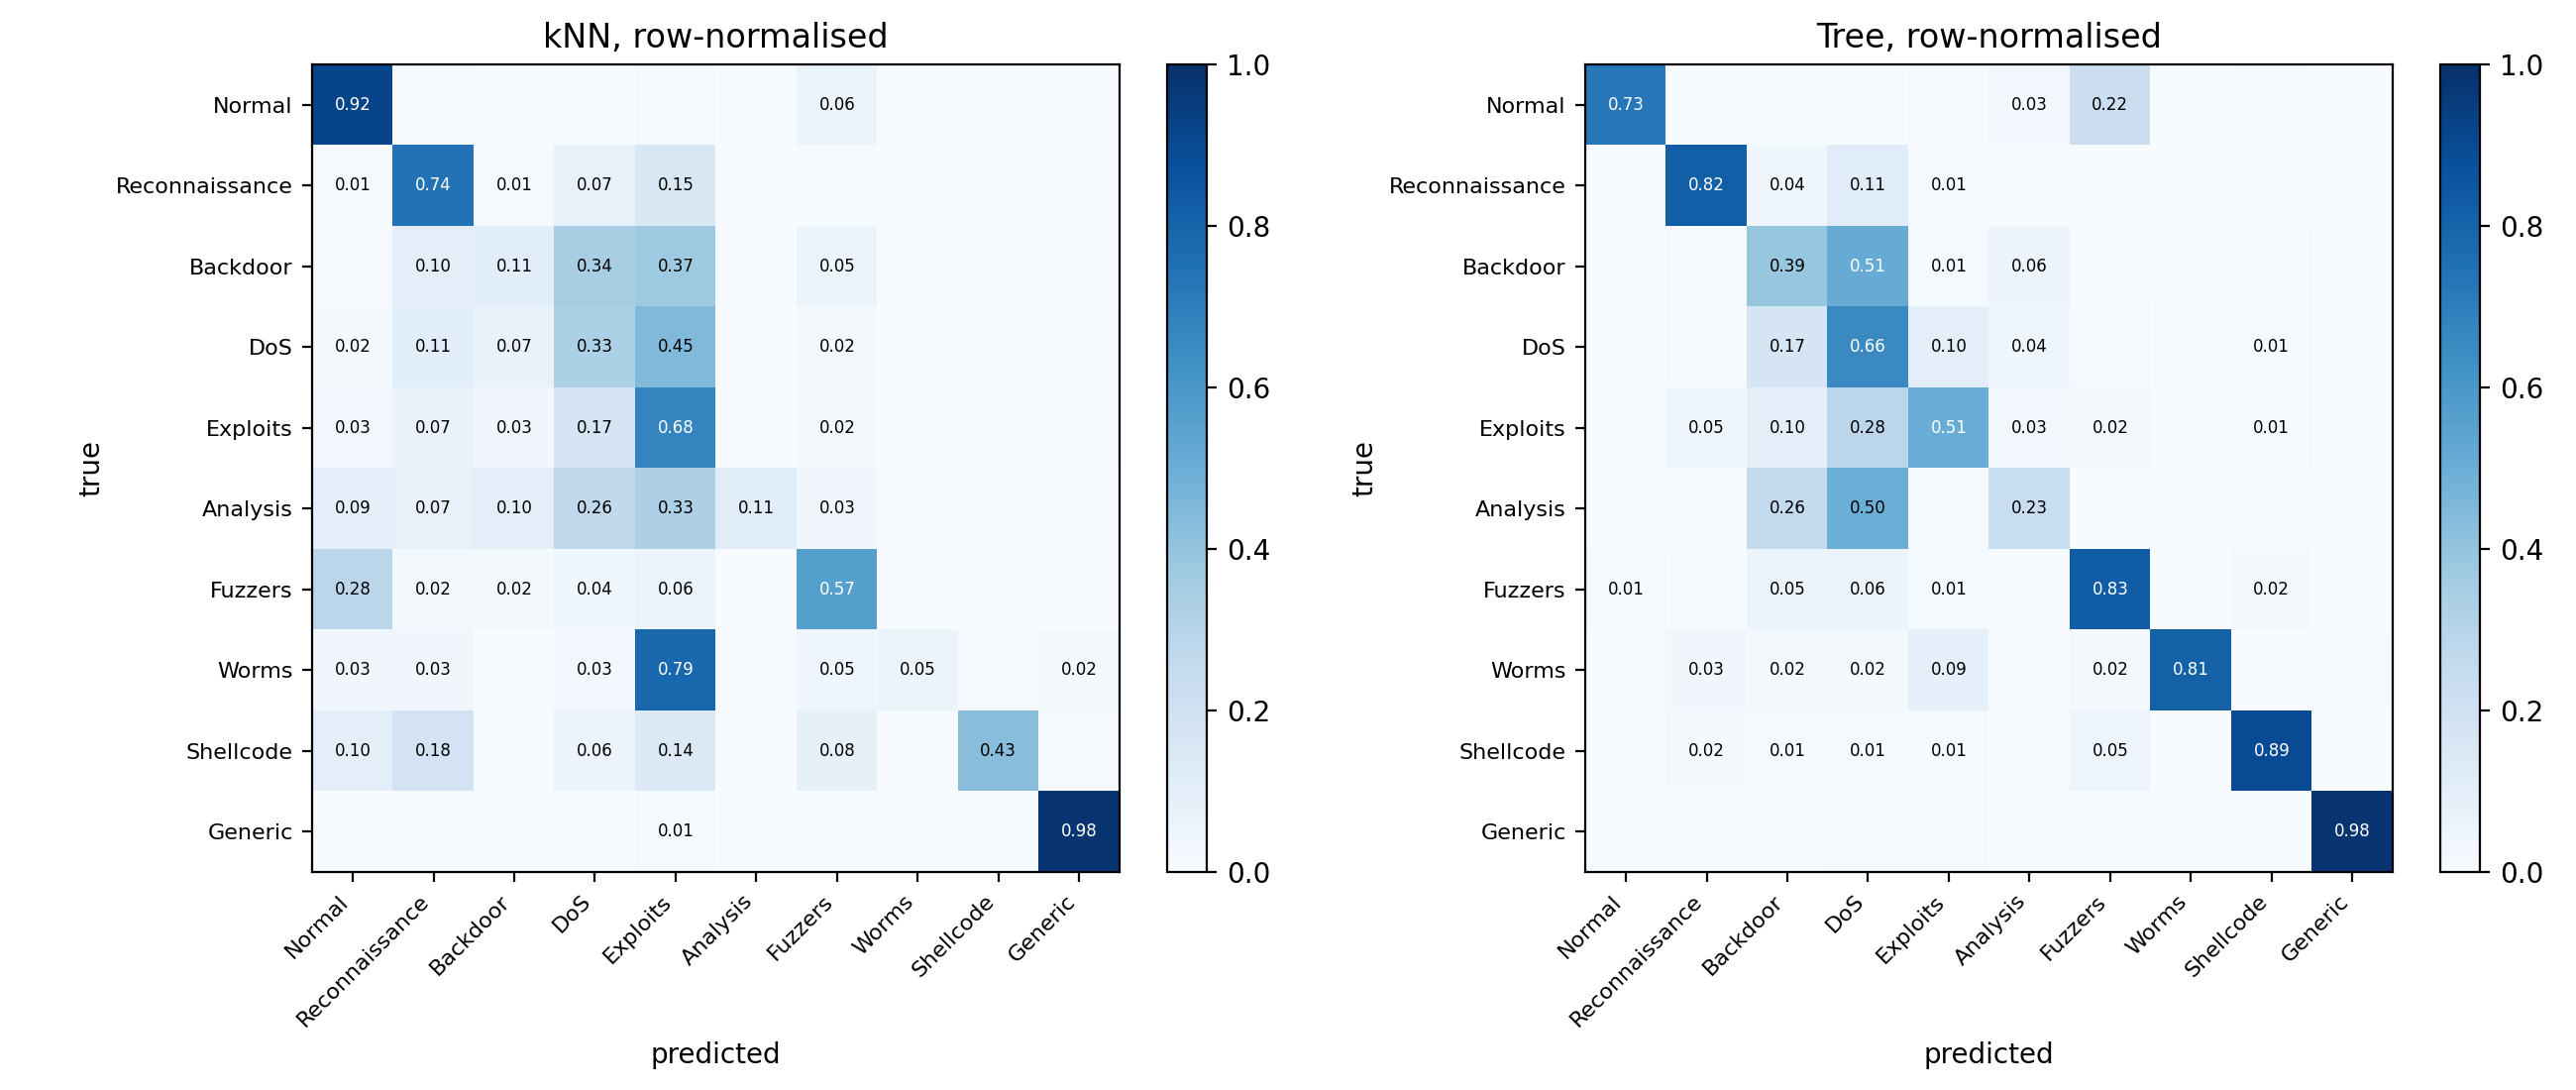
\includegraphics[width=1\textwidth]{figures/confusion_matrices.png}
\caption{Confusion matrices for the classification tree and for the nearest
neighbour model}
\label{fig:cm}
\end{figure*}

\subsection{Per-Class Performance}
\label{sec:perclass}

Table~\ref{tab:perclass} gives the per-class F1 of both models against the
ceiling imposed by the conflicting labels. Reading the weak classes as a single
group would be a mistake, because they are weak for two different reasons, and
the two call for different remedies.

\begin{table}[t]
\caption{Per-class F1 against the achievable ceiling}
\label{tab:perclass}
\centering
\begin{tabular}{l r r r}
\toprule
Class & Classification tree & $k$-nearest neighbours & Ceiling \\
\midrule
Normal          & 0.839 & 0.913 & 0.997 \\
Generic         & 0.987 & 0.985 & 0.997 \\
Reconnaissance  & 0.823 & 0.672 & 0.913 \\
Exploits        & 0.637 & 0.675 & 0.817 \\
Fuzzers         & 0.607 & 0.606 & 0.914 \\
Worms           & 0.576 & 0.067 & 0.954 \\
Shellcode       & 0.528 & 0.463 & 0.998 \\
DoS             & 0.464 & 0.328 & 0.528 \\
Analysis        & 0.149 & 0.188 & 0.375 \\
Backdoor        & 0.139 & 0.079 & 0.261 \\
\bottomrule
\end{tabular}
\end{table}

Backdoor, Analysis and DoS are limited by the data itself, since their ceilings are 
0.261, 0.375 and 0.528, so no classifier can achieve a high score on these classes. 
Measured against what is actually achievable, the tree performs reasonably well 
on DoS, with a score of 0.464, which is 88\% of the available 0.528. The 
confusion matrix shows that these three classes are often confused with each 
other, with 51.0\% of Backdoor instances and 49.7\% of Analysis instances
predicted as DoS.
This is mainly due to the features available. Every descriptive feature is a 
connection-level statistic, covering duration, byte and packet counts, timing 
and protocol flags. None of them describes what the attacker was trying to do. 
If two attacks have different intentions but produce similar connection patterns, 
the models cannot distinguish them because that information is not present in the 
features.

Shellcode and Worms have the opposite problem. Their ceilings are 0.998 and
0.954, so both are almost perfectly separable, but the evaluation pool holds
only 1\,335 and 154 instances of them. The weakness is representation rather
than separability, so more examples would help, whereas additional data would
not solve the feature limitation affecting Backdoor and Analysis.

Set against the ceiling, the tree reached 74\% of the achievable macro F1 and
kNN 64\%. The distance between the two models is therefore smaller than the
distance between either model and the limit of the data.

\subsection{Confirmation of the Stated Expectations}
\label{sec:expectconfirm}

The prediction about Worms in Section~\ref{sec:expectations} held. kNN scored
an F1 of 0.067 on the class, recovering 5.2\% of its instances and sending
78.6\% of them to Exploits. With a class that small a Worms query rarely holds
even one Worms instance among its three nearest neighbours, and
KNeighborsClassifier offers no class weighting to compensate, which is the
predicted outcome of a sufficiently imbalanced dataset letting the majority
level dominate despite distance weighting \cite{kelleher2015}. The tree, which
could be weighted, reached 0.576 with a recall of 81.2\%.

Weighting was not free. The tree bought its recall by spending precision, ending
with a macro recall of 0.684 against a macro precision of 0.554. Backdoor shows
the trade at its most extreme: the tree predicted the class 9\,551 times for
2\,058 actual instances, roughly four and a half times too often, for a
precision of 0.084 against a recall of 0.392. A model tuned on macro F1 accepts
that exchange because finding a rare attack usually matters more than
occasionally raising a false alarm.

The expectation about nominal encoding was not supported. One-hot encoding
reached 0.5143 against 0.4991 for ordinal encoding under the selected criterion
and weighting, a margin of roughly one standard deviation, and one-hot won three
of the four criterion and weighting combinations tested. The reasoning in
Section~\ref{sec:expectations} overlooked how the split is actually found. The
best split for an enumerated attribute with $k$ values lies at one of the $k-1$
positions obtained by ordering the levels by their average class value
\cite{wang1997}, but OrdinalEncoder orders levels alphabetically. Across 133
protocol levels the tree was therefore searching 132 cut points in an
essentially arbitrary ordering, which is worse than searching 133 binary
features.

Query cost behaved as the lazy learning argument of
Section~\ref{sec:algorithms} predicts. kNN needed 316.5 seconds per fold
against 0.07 seconds for the tree, a difference of more than three orders of
magnitude \cite{kelleher2015}.

% ============================================================
\section{Conclusions}
\label{sec:conclusion}

This report compared $k$-nearest neighbours (kNN) with a classification tree on a 
ten-class network intrusion detection problem. Pre-processing was selected 
separately for each model, with control parameters tuned using grid search on a 
separate pool of 30\,000 instances. Both models were then evaluated using 
ten-fold stratified cross-validation on the remaining 227\,673 instances.

Overall, the classification tree was the better model. It achieved a higher 
macro F1 of 0.5749 compared with 0.4975, performed better on average class accuracy 
using both the arithmetic and harmonic means, and achieved higher F1 scores for 
seven of the ten classes. It was also more than three orders of magnitude 
faster at prediction time. The tree won all ten folds, and the difference 
remained significant under the corrected resampled $t$-test, not just the 
uncorrected version.

There is one important qualification. kNN achieved higher plain accuracy and
weighted F1, but both metrics are dominated by the two largest classes, whereas
macro F1 gives the rare attack classes equal importance. For intrusion
detection that is the more useful priority, but it remains a choice of
evaluation priority rather than an objective property of the dataset.

Two expectations drawn from theory were not supported. Removing correlated
features was expected to improve kNN, and ordinal encoding was expected to suit
the tree better than one-hot encoding. Neither held, and both were caught
because the choices were tested during tuning.

The binding constraint is the data itself. The tree reached only 74\% of the
macro F1 ceiling imposed by the conflicting labels, so further work should begin
with features that separate Backdoor, Analysis and DoS, which connection-level
statistics alone cannot distinguish. A similarity index that ignores co-absences
would suit the sparse binary features produced by one-hot encoding
\cite{kelleher2015}, and a k-d tree index would cut the query cost if kNN were
ever deployed \cite{kelleher2015}. Any deployed model would also need continued
validation, since attack traffic changes over time and models are subject to
concept drift \cite{kelleher2015}.

% ============================================================
\begin{thebibliography}{9}

\bibitem{topic3}
A. P. Engelbrecht, ``Similarity-based learning,'' Topic 3 lecture notes, Machine
Learning 741, Stellenbosch University, 2026.

\bibitem{topic4}
A. P. Engelbrecht, ``Information-based learning,'' Topic 4 lecture notes, Machine
Learning 741, Stellenbosch University, 2026.

\bibitem{kelleher2015}
J. D. Kelleher, B. Mac Namee, and A. D'Arcy, \textit{Fundamentals of Machine
Learning for Predictive Data Analytics: Algorithms, Worked Examples, and Case
Studies}. Cambridge, MA: MIT Press, 2015, pp. 162--174, 182, 184--188,
196--199, 221, 230--233, 241--245, 251--254, 263--269, 426--427, 432--438,
442--445, 464, 472.

\bibitem{rodden2000}
K. Rodden, W. Basalaj, D. Sinclair, and K. Wood, ``A comparison of measures for
visualising image similarity,'' in \textit{Proceedings of the Challenge of Image
Retrieval}, 2000.

\bibitem{wickramarachchi2016}
D. C. Wickramarachchi, B. L. Robertson, M. Reale, C. J. Price, and J. Brown,
``HHCART: an oblique decision tree,'' \textit{Computational Statistics and Data
Analysis}, vol. 96, pp. 12--23, 2016.

\bibitem{wang1997}
Y. Wang and I. H. Witten, ``Inducing model trees for continuous classes,'' in
\textit{Proceedings of the Poster Papers of the European Conference on Machine
Learning}, 1997.

\end{thebibliography}

\end{document}